\documentclass[11pt]{article}
\usepackage[margin=1.05in]{geometry}
\usepackage{amsmath,amssymb,amsthm,mathtools}
\usepackage{booktabs,microtype,xcolor,graphicx}
\usepackage[shortlabels]{enumitem}
\usepackage[colorlinks=true,linkcolor=blue!45!black,citecolor=blue!45!black,urlcolor=blue!45!black]{hyperref}
\hypersetup{pdftitle={What the visit counts remember},pdfauthor={Arjun Pemmasani}}
\newtheorem{theorem}{Theorem}[section]
\newtheorem{lemma}[theorem]{Lemma}
\newtheorem{proposition}[theorem]{Proposition}
\newtheorem{corollary}[theorem]{Corollary}
\theoremstyle{definition}
\newtheorem{example}[theorem]{Example}
\theoremstyle{remark}
\newtheorem{remark}[theorem]{Remark}
\newcommand{\E}{\mathbb E}
\newcommand{\Prob}{\mathbb P}
\newcommand{\C}{\mathbb C}
\newcommand{\one}{\mathbf 1}
\emergencystretch=1.5em
\title{What the visit counts remember\\[4pt]
\large Working note for direction S2 (independent derivation, not yet compared with the S2 notes)}
\author{}
\date{October 2026}
\begin{document}
\maketitle

\section{The question and the answer}

A chain on $d$ states switches slowly. We do not see its path. We only see how
long it spent in each state (the count vector of Paper~C, divided by $N$). Which
rate matrices can be told apart from this, and how much is lost compared with
seeing the path?

Here is what we find. The proofs are in the sections that follow.
\begin{enumerate}[1.,itemsep=2pt]
\item \emph{One horizon is every horizon} (Theorem~\ref{thm:horizon}). The law of
 the counts at a single time fixes their law at every time.
\item \emph{The counts know each pair of flows, but not which is which}
 (Theorem~\ref{thm:pairs}). For two states $i$ and $j$, the counts fix the flow
 from $i$ to $j$ and the flow from $j$ to $i$ as an unordered pair. The exit
 rates then decide the order for almost every chain, so almost every chain can be
 recovered (Corollary~\ref{cor:generic}).
\item \emph{A stationary start hides the arrow of time, and nothing else}
 (Proposition~\ref{prop:reversal}, Theorem~\ref{thm:rigid}). A chain and its
 reversal give the same counts. These are the only two candidates whenever the
 rate matrix has no cut (no way to split the states into two groups of two or
 more that talk to each other through rank one blocks), and almost every chain
 is like this. The size of the net flow on every pair is still known, so the
 counts say how far the chain is from reversible but not which way it turns.
\item \emph{The counts measure the entropy production}
 (Theorem~\ref{thm:entropy}). They cannot tell a film of the chain from the
 same film run backward. Yet they determine exactly how different the two films
 are, namely the entropy production rate, and from any start they decide
 whether the chain is reversible (when every rate is positive).
\item \emph{Lumping gives more ties} (Theorem~\ref{thm:lumping}). If a group of
 states looks like a single state from outside, we can reverse the outside and
 keep the inside, or reverse the inside and keep the outside. This gives two
 chains on four states, with every rate positive and a start that is not
 stationary, that no amount of count data can tell apart.
\item \emph{What is lost} (Theorems~\ref{thm:info} and~\ref{thm:singular}). When
 switches are rare, the counts are as good as the full path for the two-way flow
 on each pair, and blind to first order to the net flow. With a stationary start
 the information about the net flow vanishes exactly at reversible chains, at
 every horizon.
\end{enumerate}

\section{Setting}

Let $G=(g_{ij})$ be a rate matrix on $[d]=\{1,\ldots,d\}$, so $g_{ij}\ge0$ for
$i\ne j$ and $q_i=-g_{ii}=\sum_{j\ne i}g_{ij}$ is the exit rate of $i$. Let $Y$
be the chain with rates $G$ and start law $\mu$, and let
\[
L_i(t)=\int_0^t\one\{Y_s=i\}\,ds,\qquad L(t)=(L_1(t),\ldots,L_d(t)).
\]
This is the limit of Paper~C's setting. If $X$ is the $N$-step chain with
transition matrix $I+G/N$, then its count vector $K_N$ satisfies $K_N/N\to L(1)$
in law. With $G=TQ$ the number $T$ counts the switches, as in Papers~A to~C.

We use three numbers for each pair of states. The \emph{flows} are
$f_{ij}=\mu_ig_{ij}$ (how much mass moves from $i$ to $j$ at time $0$). The
\emph{two-way flow} is $c_{ij}=f_{ij}+f_{ji}$ and the \emph{net flow} is
$J_{ij}=f_{ij}-f_{ji}$. We also write $a_{ij}=g_{ij}g_{ji}$, the weight of a
round trip. Note that
\begin{equation}\label{eq:roots}
f_{ij}+f_{ji}=c_{ij},\qquad f_{ij}f_{ji}=\mu_i\mu_ja_{ij},\qquad
J_{ij}^2=c_{ij}^2-4\mu_i\mu_ja_{ij},
\end{equation}
and that $\sum_jJ_{ij}=-(\mu G)_i$. So $\mu$ is stationary exactly when the net
flow obeys Kirchhoff's law at every state, and the chain is reversible with
respect to $\mu$ exactly when $J=0$. (In the physics literature $c_{ij}$ is the
traffic or dynamical activity of the pair and $J_{ij}$ is its current, and the
times $L$ are the standard example of an observable that does not change when
time is reversed~\cite{mnw2008}.)

Write $\Lambda=\operatorname{diag}(\lambda)$. By the Feynman--Kac formula, for
$\lambda\in\C^d$,
\begin{equation}\label{eq:FK}
\Phi_t(\lambda)=\E\,e^{-\lambda\cdot L(t)}=\mu^{\top}e^{t(G-\Lambda)}\one,
\qquad
r(\lambda)=\int_0^\infty\Phi_t(\lambda)\,dt=\mu^{\top}(\Lambda-G)^{-1}\one ,
\end{equation}
the second for $\lambda$ with positive coordinates. The function $r$ is rational,
which is what makes it easy to read.

\begin{proposition}[reversal]\label{prop:reversal}
Let $\mu=\pi$ be stationary for $G$ with $\pi_i>0$, and let
$\hat g_{ij}=\pi_jg_{ji}/\pi_i$. Then $(\pi,\hat G)$ and $(\pi,G)$ give the same
law of $L(t)$ for every $t$.
\end{proposition}
\begin{proof}
Run the film backward. The path $s\mapsto Y_{t-s}$ is the stationary chain with
rates $\hat G$, and it spends the same time in each state as $Y$ does.
\end{proof}

In terms of flows, reversal swaps $f_{ij}$ and $f_{ji}$ on every pair. So it
keeps $c$ and flips the sign of $J$.

\section{One horizon is every horizon}

\begin{theorem}\label{thm:horizon}
Let $G$ be irreducible. Suppose a second pair $(\mu',G')$ gives the same law of
$L(1)$. Then it gives the same law of $L(t)$ for every $t>0$, and $r'=r$.
\end{theorem}

The idea is that each state contributes one mode $e^{z_i(\lambda)}$ to
$\Phi_1$, where $z_i$ is an eigenvalue of $G-\Lambda$. Exponentials of different
algebraic functions cannot cancel each other, so each mode can be read off from
$\Phi_1$. The modes are the poles of the resolvent, and the resolvent knows every
horizon. We need two lemmas. Both are known. The first is a weak case of
theorems on the independence of exponentials~\cite{ax1971}, and the second is
Lemma~5.1 of~\cite{alahmadieh2026}. We include short proofs.

\begin{lemma}[exponentials do not cancel]\label{lem:exp}
Let $B\subset\C^d$ be a ball and let $w_1,\ldots,w_m$ and $c_1,\ldots,c_m$ be
holomorphic functions on $B$ that are algebraic over $\C(\lambda)$. Suppose
$w_a-w_b$ is not constant for $a\ne b$. If $\sum_ac_ae^{w_a}=0$ on $B$, then
every $c_a$ is zero.
\end{lemma}
\begin{proof}
We use induction on $m$. The case $m=1$ is clear. Suppose the claim holds for
$m-1$ and that $c_m\ne0$ (otherwise we have fewer terms). On a smaller ball
where $c_m$ has no zero, divide by $c_me^{w_m}$ and differentiate in
$\lambda_j$. With $b_a=c_a/c_m$ and
$v_a=w_a-w_m$ this gives
$\sum_{a<m}(\partial_jb_a+b_a\partial_jv_a)e^{v_a}=0$, which has $m-1$ terms. By
induction $\partial_j(b_ae^{v_a})=0$ for every $j$ and every $a<m$, so
$b_ae^{v_a}$ is a constant $k_a$. If some $k_a\ne0$, then $e^{v_a}=k_a/b_a$ is
algebraic. This is impossible. Restrict to a complex line on which $v_a$ is not
constant. There $v_a$ is a nonconstant meromorphic function on a compact Riemann
surface, so it has a pole, and near the pole $e^{v_a}$ has an essential
singularity, which an algebraic function does not have. Hence every $k_a=0$, so
$c_a=0$ for $a<m$ (on the smaller ball, and so on $B$), and then $c_m=0$, which
contradicts our assumption.
\end{proof}

\begin{lemma}[one polynomial]\label{lem:irred}
If $G$ is irreducible, then $\chi(z,\lambda)=\det(z+\Lambda-G)$ is an irreducible
polynomial.
\end{lemma}
\begin{proof}
We argue by contradiction. A factorization of $\chi$ would force a product rule
on its coefficients, and a cycle of the chain breaks that rule.

Put $x_i=z+\lambda_i+q_i$, let $X=\operatorname{diag}(x_1,\ldots,x_d)$, and let
$A\ge0$ be $G$ without its diagonal. Then
\[
\chi=\det(X-A)=\sum_{U\subseteq[d]}m(U)\prod_{i\notin U}x_i,
\qquad m(U)=\det(-A_{UU}),\quad m(\emptyset)=1 .
\]
So $\chi$ is a polynomial in $x_1,\ldots,x_d$ alone, and it is enough to show
that it does not factor as such a polynomial. (Use $x_1,\ldots,x_d$ and $z$ as
coordinates. Then $\chi$ has degree zero in $z$, so every factor of $\chi$ does
too.) It has degree exactly one in
each $x_i$. Suppose $\chi=\chi_1\chi_2$ with both factors nonconstant. Then each
$x_i$ appears in exactly one factor, so the variables split into two nonempty
sets $S$ and $S^c$, with $\chi_1$ using only $S$ and $\chi_2$ only $S^c$. Scale
the factors so that each has top coefficient $1$. Comparing coefficients gives
\[
m(U\cup V)=m(U)\,m(V)\qquad\text{for }U\subseteq S\text{ and }V\subseteq S^c .
\]

Since $G$ is irreducible, some cycle of positive rates meets both $S$ and $S^c$.
Take one with the fewest states, let $W$ be its set of states, and put
$U=W\cap S$, $V=W\cap S^c$. Expand $m(W)$ over permutations of $W$. The
permutations that keep $U$ and $V$ apart sum to $m(U)m(V)$. Any other permutation
with nonzero weight contains a cycle that meets both sides, which by our choice
uses all of $W$. A single cycle on $W$ has sign $(-1)^{|W|-1}$ and weight
$(-1)^{|W|}$ times a product of rates, so it contributes minus that product.
These contributions all have the same sign, so they cannot cancel, and ours is
not zero. So $m(W)\ne m(U)m(V)$, a contradiction.
\end{proof}

\begin{proof}[Proof of Theorem~\ref{thm:horizon}]
We write $\Phi_1$ as a sum of $d$ exponentials on a ball where the eigenvalues
of $G-\Lambda$ are far apart, do the same for $\Phi_1'$, and match the two sums
term by term.

Both $\Phi_1$ and $\Phi_1'$ are entire and agree on $\mathbb R^d$, so they agree
on $\C^d$. Let $m=2\max_i\max(q_i,q_i')$ and let $B$ be the ball of radius $3m$
around the real point $(0,12m,24m,\ldots)$. On $B$ we have
$|\lambda_i-\lambda_j|>6m$ for $i\ne j$. By Gershgorin's theorem, the matrix
$G-\Lambda$ then has exactly one eigenvalue $z_i(\lambda)$ in the disc
$|z+\lambda_i+q_i|\le q_i$ for each $i$, and these discs are disjoint. So the
$z_i$ are simple, holomorphic and algebraic on $B$, and
\[
\Phi_1=\sum_i\rho_ie^{z_i},\qquad
\rho_i=\frac{n(z_i,\lambda)}{\partial_z\chi(z_i,\lambda)},\qquad
n(z,\lambda)=\mu^{\top}\operatorname{adj}(z+\Lambda-G)\one,
\]
where $\rho_i$ is the residue of $n/\chi=\mu^{\top}(z+\Lambda-G)^{-1}\one$ at
$z_i$. Since the residues of a resolvent sum to the identity, $\sum_i\rho_i=1$.
The same holds for $(\mu',G')$ with $z_i'$, $\rho_i'$ and $\chi'$.

We now compare the two expansions of $\Phi_1$ in three steps.

\emph{No mode is missing.} We claim that no $\rho_i$ vanishes identically on
$B$. If one did, then $n(z_i(\lambda),\lambda)=0$ on $B$, so $n$ and $\chi$
would share the root $z_i$ and hence a common factor. Since $\chi$ is
irreducible (Lemma~\ref{lem:irred}), it would divide $n$. But $n$ has degree
$d-1$ in $z$, less than $\chi$, and it is not zero, because its leading
coefficient in $z$ is $\sum_i\mu_i=1$.

\emph{The modes match.} On $B$ we have $|z_i+\lambda_i|\le m$ and
$|z_j'+\lambda_j|\le m$, so each of the differences $z_i-z_j$, $z_i'-z_j'$ and
$z_i-z_j'$ stays within $2m$ of $\lambda_j-\lambda_i$. For $i\ne j$ the number
$\lambda_j-\lambda_i$ moves by more than $4m$ across $B$. So none of these
differences with $i\ne j$ is constant, and the only exponents that can differ
by a constant are $z_i$ and $z_i'$ with the same $i$. Now
$\sum_i\rho_ie^{z_i}-\sum_i\rho_i'e^{z_i'}=0$ on $B$. Merge $z_i$ and $z_i'$
into one term whenever they differ by a constant, and apply
Lemma~\ref{lem:exp}. Every coefficient is then zero. If $z_i$ were not merged,
its coefficient would be $\rho_i$, which is not zero. So $z_i'=z_i-\kappa_i$
for a constant $\kappa_i$, the merged coefficient is
$\rho_i-e^{-\kappa_i}\rho_i'$, and hence $\rho_i'=e^{\kappa_i}\rho_i$.

\emph{The constants vanish.} The polynomials $\chi'(z,\lambda)$ and
$\chi(z+\kappa_1,\lambda)$ share the root $z_1-\kappa_1$ on $B$. The second is
irreducible, so it divides the first. Both have degree $d$ in $z$ with leading
coefficient $1$, so they are equal. Their roots are the $z_i-\kappa_i$ and the
$z_i-\kappa_1$. So $z_i-\kappa_i=z_j-\kappa_1$ for some $j$, and $j=i$ because
$z_i-z_j$ is not constant for $j\ne i$. Thus $\kappa_i=\kappa_1$ for every $i$.
Then $1=\sum_i\rho_i'=e^{\kappa_1}\sum_i\rho_i=e^{\kappa_1}$. Also $\kappa_1$ is
real. (At the center of $B$ the matrices are real, and each disc contains one
eigenvalue and is symmetric about the real axis, so $z_1$ and $z_1'$ are real
there.) Hence $\kappa_1=0$, and every $\kappa_i=0$.

So $\chi'=\chi$ and $\rho_i'=\rho_i$, which gives
$\mu'^{\top}(z+\Lambda-G')^{-1}\one=\sum_i\rho_i/(z-z_i)=\mu^{\top}(z+\Lambda-G)^{-1}\one$
on $B$, and so everywhere, since both sides are rational. The left and right
sides are the Laplace transforms in $t$ of $\Phi_t'$ and $\Phi_t$. Hence
$\Phi_t'=\Phi_t$ for every $t$, and $z=0$ gives $r'=r$.
\end{proof}

\section{What the counts know about a pair}

\begin{theorem}\label{thm:pairs}
Let $G$ be irreducible and $\mu_i>0$ for every $i$. The law of $L(1)$ determines
$\mu_i$ and $q_i$ for every state, and $a_{ij}$ and $c_{ij}$ for every pair. So
by~\eqref{eq:roots} it determines $\{f_{ij},f_{ji}\}$ as an unordered pair,
namely the two roots of $x^2-c_{ij}x+\mu_i\mu_ja_{ij}$, and with it $|J_{ij}|$.
\end{theorem}
\begin{proof}
By Theorem~\ref{thm:horizon} the law determines $r$. For a set $F$ of states let
$\lambda_k\to\infty$ for every $k\notin F$. Then $e^{-\lambda\cdot L(t)}$
decreases to $e^{-\lambda\cdot L(t)}\one\{Y\text{ stays in }F\text{ up to }t\}$,
so $r$ tends to $r_F=\mu_F^{\top}(\Lambda_F-G_{FF})^{-1}\one$, the same function
for the chain killed when it leaves $F$. With $x_i=\lambda_i+q_i$,
\[
r_{\{i\}}=\frac{\mu_i}{x_i},\qquad
r_{\{i,j\}}=\frac{\mu_ix_j+\mu_jx_i+c_{ij}}{x_ix_j-a_{ij}} .
\]
The first gives $\mu_i$ and $q_i$. In the second, cross-multiplying two such
fractions and comparing the coefficients of $x_ix_j$ and then of $x_i$ shows
that $c_{ij}$ and $a_{ij}$ are determined.
\end{proof}

The formula for $r_{\{i,j\}}$ says what is going on. A path that jumps once
between $i$ and $j$ leaves the same counts whether it went from $i$ to $j$ at
time $s$ or from $j$ to $i$ at time $1-s$. So one-jump paths show only the sum
$c_{ij}$. Round trips show the product $a_{ij}$. A sum and a product give two
numbers, but not their order.

Let $S$ be a set of pairs. Write $G^S$ for the matrix obtained from $G$ by
swapping $f_{ij}$ and $f_{ji}$ on every pair in $S$ (so
$g^S_{ij}=\mu_jg_{ji}/\mu_i$ there), with the diagonal chosen so that rows sum
to zero.

\begin{corollary}[the exit rates decide]\label{cor:candidates}
Under the hypotheses of Theorem~\ref{thm:pairs}, every $(\mu',G')$ with the same
law of $L(1)$ has $\mu'=\mu$ and $G'=G^S$ for a set $S$ of pairs on which the
net flow obeys Kirchhoff's law,
\begin{equation}\label{eq:kirchhoff}
\sum_{j:\{i,j\}\in S}J_{ij}=0\qquad\text{for every state }i .
\end{equation}
\end{corollary}
\begin{proof}
By Theorem~\ref{thm:pairs}, $G'$ has the same $\mu$, the same exit rates and the
same unordered pairs of flows. Let $S$ be the set of pairs where the order
differs. The exit rate of $i$ is $\sum_jf_{ij}/\mu_i$, and swapping changes it by
$-\sum_{j:\{i,j\}\in S}J_{ij}/\mu_i$.
\end{proof}

\begin{corollary}\label{cor:generic}
Let $G$ be irreducible and $\mu_i>0$ for every $i$.
\begin{enumerate}[(a),itemsep=1pt]
\item If $d=2$, the law of $L(1)$ determines $(\mu,G)$.
\item If $d=3$, it determines $(\mu,G)$ unless $\mu$ is stationary and the chain
 is not reversible. In that case exactly two pairs have this law, namely
 $(\mu,G)$ and its reversal.
\item For every $\mu$ and almost every $G$, it determines $(\mu,G)$.
\item If $d\ge3$ and $\mu$ is the stationary law, then for almost every $G$
 exactly two pairs have this law, namely $(\mu,G)$ and its reversal.
\end{enumerate}
\end{corollary}
\begin{proof}
By Corollary~\ref{cor:candidates} we only have to find the sets $S$ that
satisfy~\eqref{eq:kirchhoff}. Swapping a pair with $J_{ij}=0$ changes nothing,
so we may take $J_{ij}\ne0$ on $S$.

(a) A single pair with $J_{12}\ne0$ cannot satisfy~\eqref{eq:kirchhoff}. So $S$
is empty and $G'=G$.

(b) A state that lies in exactly one pair of $S$
violates~\eqref{eq:kirchhoff}. With three states this leaves only $S$ empty or
$S$ all three pairs. In the second case~\eqref{eq:kirchhoff} gives
$J_{12}=J_{23}=J_{31}\ne0$. Then $\sum_jJ_{ij}=0$ at every state, so $\mu$ is
stationary and the chain is not reversible. Also $G^S$ is the reversal, and
Proposition~\ref{prop:reversal} shows that it does have the same law.

(c) Fix $\mu$ and use the flows $f_{ij}$ as coordinates for $G$. For each
nonempty $S$, condition~\eqref{eq:kirchhoff} at a state that meets $S$ is a
linear equation in the flows that is not trivial. So it fails off a hyperplane,
and off these finitely many hyperplanes only $S$ empty is left.

(d) Use the coordinates $(\pi,c,J)$, where $J$ runs over the flows that obey
Kirchhoff's law on the whole graph. Let $S$ be neither empty nor everything.
Some state $i$ has a pair $\{i,j\}$ in $S$ and a pair $\{i,k\}$ outside it. The
unit flow around the triangle $i\to j\to k\to i$ is an allowed $J$, and it
violates~\eqref{eq:kirchhoff} at $i$, because only its edge $\{i,j\}$ counts
there. So~\eqref{eq:kirchhoff} at $i$ is again a linear equation that is not
trivial, and it fails off a proper subspace. What is left is $S$ empty or
everything, which gives $G$ and its reversal. These two differ unless $J=0$.
(For $d=2$ every chain is reversible, so there the two coincide.)
\end{proof}

\begin{remark}
The proof is also a recipe. Read $\mu_i$ and $q_i$ from the paths that never
move, and $c_{ij}$ and $a_{ij}$ from the paths that visit two states. Then
$f_{ij}=\frac12(c_{ij}\pm|J_{ij}|)$, and the signs are the ones for which
$\sum_jf_{ij}=\mu_iq_i$ at every state. So paths that visit at most two states
are enough for almost every chain.
\end{remark}

\begin{remark}
Part (d) is sharper than ``the counts cannot see irreversibility''. They cannot
see its direction. They do see $|J_{ij}|$ on every pair, so they know exactly
how far the chain is from reversible. For long horizons it is known that the
variance of $L$ and its large deviations depend on the net flow only through
even expressions~\cite{dlp2016,kjz2017}. Here the statement is exact, at every
horizon, and for the whole law.
\end{remark}

\section{Chains without a cut}\label{sec:rigid}

Theorem~\ref{thm:pairs} reads the law through the paths that visit at most two
states. Reading all of it leads to an old question of linear algebra, namely
when two matrices have the same principal minors.

\begin{proposition}[two sets of minors]\label{prop:minors}
Let $G$ be irreducible. The law of $L(1)$ determines every principal minor of
$G$ and every principal minor of $G-\one\mu^{\top}$. Conversely, these minors
determine the law of $L(t)$ for every $t$.
\end{proposition}
\begin{proof}
The law determines the rational function $r$. We show that its denominator
and its numerator can be read off separately, and that their coefficients are
the two sets of minors.

By Theorem~\ref{thm:horizon} the law determines $r=n_0/\chi_0$, where
\[
\chi_0(\lambda)=\det(\Lambda-G),\qquad
n_0(\lambda)=\mu^{\top}\operatorname{adj}(\Lambda-G)\one .
\]
The polynomial $\chi_0$ is irreducible (the proof of Lemma~\ref{lem:irred} with
$z=0$). The polynomial $n_0$ is not zero and has smaller degree, so $\chi_0$
does not divide it. Hence the fraction is in lowest terms, and $r$ determines
$\chi_0$ and $n_0$ up to a common constant factor. The factor is fixed because
the coefficient of $\lambda_1\cdots\lambda_d$ in $\chi_0$ is $1$. (A second
pair $(\mu',G')$ with the same law has $r'=r$, with a denominator of the same
degree and the same top coefficient. So $\chi_0'=\chi_0$ and $n_0'=n_0$, and we
do not need $G'$ to be irreducible.)

Now we read the coefficients. For a matrix $A$ we have
$\det(\Lambda-A)=\sum_{U}\det(-A_{UU})\prod_{i\notin U}\lambda_i$. With $A=G$
this is $\chi_0$, so the coefficients of $\chi_0$ are the principal minors of
$-G$, which are those of $G$ up to the sign $(-1)^{|U|}$. Next, the rule for
the determinant of a rank one change gives
$\det(\Lambda-G+\one\mu^{\top})=\chi_0+n_0$. So the coefficients of
$\chi_0+n_0$ are the principal minors of $-(G-\one\mu^{\top})$.

For the converse, the two sets of minors give $\chi_0$ and $\chi_0+n_0$, and so
$r$. Since the coordinates of $L(t)$ sum to $t$, we have
$\Phi_t(\lambda+z\one)=e^{-zt}\Phi_t(\lambda)$. So $z\mapsto r(\lambda+z\one)$
is the Laplace transform of $t\mapsto\Phi_t(\lambda)$, and it determines
$\Phi_t(\lambda)$ for every $t$.
\end{proof}

For example, the sets $U$ with one element give $q_i$ from the first set of
minors and $q_i+\mu_i$ from the second. So the second set is where the start
law enters.

Two things always keep the principal minors of a matrix $A$, namely passing to
$DAD^{-1}$ for a diagonal matrix $D$ and passing to the transpose. For a rate
matrix these are familiar. The transpose with the right $D$ is the reversal,
since $\hat G=\Pi^{-1}G^{\top}\Pi$ with $\Pi=\operatorname{diag}(\pi)$. Hartfiel
and Loewy~\cite{hl1984} and Loewy~\cite{loewy1986} found when nothing else keeps
them. Say that $G$ has a \emph{cut} if there is a set $X$ of states with
$2\le|X|\le d-2$ such that both blocks $G_{XX^c}$ and $G_{X^cX}$ have rank at
most one. (So a chain on two or three states has no cut.) Their theorem says
that if $A$ is irreducible and has no cut, then every matrix with the same
principal minors as $A$ is $DAD^{-1}$ or $DA^{\top}D^{-1}$ for some diagonal $D$
(see also~\cite[Theorem~4.1]{alahmadieh2026}).

\begin{theorem}[at most two candidates]\label{thm:rigid}
Let $G$ be irreducible with no cut, and let $\pi$ be its stationary law. Suppose
$(\mu',G')$ gives the same law of $L(1)$ as $(\mu,G)$. Then $\mu'=\mu$, and
$G'$ is either $G$ or its reversal $\hat G$. Moreover $(\mu,\hat G)$ does give
the same law if and only if, for the stationary chain with rates $G$ and
$w_i=\mu_i/\pi_i$,
\begin{equation}\label{eq:startend}
\E_\pi\bigl[w(Y_0)\mid L(1)\bigr]=\E_\pi\bigl[w(Y_1)\mid L(1)\bigr].
\end{equation}
\end{theorem}

In words, a chain with no cut has at most one rival, its own reversal, and the
rival passes exactly when the counts cannot tell the first state from the last
as far as the weight $w$ is concerned. A stationary start has $w=1$, and then
\eqref{eq:startend} is clear.

\begin{proof}
The first part is linear algebra. The theorem of Hartfiel and Loewy leaves two
families of matrices, and only one member of each family is a rate matrix. The
second part runs the film backward.

\emph{The candidates.} By Proposition~\ref{prop:minors}, $G'$ has the same
principal minors as $G$. By the theorem of Hartfiel and Loewy, $G'=DGD^{-1}$ or
$G'=DG^{\top}D^{-1}$ for an invertible diagonal matrix $D$. We use that the rows
of $G'$ sum to zero, that is, $G'\one=0$. In the first case this says
$GD^{-1}\one=0$. Since $G$ is irreducible, the only vectors it sends to zero are
the multiples of $\one$. So $D$ is a multiple of the identity and $G'=G$. In
the second case $G^{\top}D^{-1}\one=0$. The only vectors that $G^{\top}$ sends
to zero are the multiples of $\pi$, so $D^{-1}$ is a multiple of $\Pi$ and
$G'=\Pi^{-1}G^{\top}\Pi=\hat G$.

\emph{The start.} By the proof of Proposition~\ref{prop:minors} the law
determines the polynomial $n_0$, and the coefficient of
$\prod_{k\ne i}\lambda_k$ in $n_0$ is $\mu_i$. So $\mu'=\mu$.

\emph{When the reversal passes.} For a bounded function $F$ we compare
$\E F(L(1))$ under $(\mu,G)$ and under $(\mu,\hat G)$. Write $\E_\pi$ for the
stationary chain with rates $G$. The chain $(\mu,G)$ is this chain with its
start reweighted, so
\[
\E_{(\mu,G)}F(L(1))=\E_\pi\bigl[w(Y_0)F(L(1))\bigr].
\]
In the same way the chain $(\mu,\hat G)$ is the stationary chain with rates
$\hat G$ weighted by $w$ at its first state (both chains have the stationary
law $\pi$). Run the film backward, as in Proposition~\ref{prop:reversal}. The
stationary chain with rates $\hat G$ becomes the stationary chain with rates
$G$, its first state becomes the last state $Y_1$, and $L(1)$ does not change.
So
\[
\E_{(\mu,\hat G)}F(L(1))=\E_\pi\bigl[w(Y_1)F(L(1))\bigr].
\]
The two right sides agree for every $F$ exactly when $w(Y_0)-w(Y_1)$ has
conditional mean zero given $L(1)$, which is~\eqref{eq:startend}.
\end{proof}

A cut asks for $2\times2$ minors to vanish, so almost every rate matrix has
none. Thus Theorem~\ref{thm:rigid} names the exceptional chains in parts (c) and
(d) of Corollary~\ref{cor:generic}. In part (c) an exceptional chain has a cut
or satisfies~\eqref{eq:startend}. In part (d) it has a cut or is reversible
(then the two candidates are the same chain). In part (c) the second case can
happen with a start that is not stationary, as we will see after
Theorem~\ref{thm:lumping}. For a chain with every rate drawn at random it does
not happen (\texttt{check\_rigidity.py}).

The same two operations, and the same theorem of Loewy, appear for the kernels
of permanental processes, which describe local times of Markov processes at
certain random times~\cite{mr2013}. What is different here is the fixed
horizon and the start law, which bring in the second matrix $G-\one\mu^{\top}$.

\section{The counts measure the entropy production}\label{sec:entropy}

A stationary start hides the arrow of time. One might guess that the counts
then say nothing about how irreversible the chain is. The opposite is true.

The \emph{entropy production rate} of the chain at time $0$ is
\[
 \sigma(\mu,G)=\sum_{i<j}(f_{ij}-f_{ji})\log\frac{f_{ij}}{f_{ji}},
 \qquad f_{ij}=\mu_ig_{ij}
\]
(see~\cite{schnakenberg1976}). A pair with $f_{ij}=f_{ji}=0$ contributes
nothing. Each term is nonnegative, and $\sigma=0$ exactly when $J=0$. For a stationary start, $t\sigma$ is the relative entropy of the
law of the path on $[0,t]$ with respect to the law of the same path run
backward. So $\sigma$ measures how far the film is from its reverse. For three
states $i,j,k$ with all six rates positive, the \emph{affinity} of the
triangle is
\[
 A_{ijk}=\log\frac{g_{ij}g_{jk}g_{ki}}{g_{ik}g_{kj}g_{ji}} ,
\]
the logarithm of the odds of going around the triangle one way and not the
other.

\begin{theorem}[irreversibility]\label{thm:entropy}
Let $G$ be irreducible, and suppose that $g_{ij}>0$ exactly when $g_{ji}>0$.
\begin{enumerate}[(a),itemsep=1pt]
\item If $\mu_i>0$ for every $i$, the law of $L(1)$ determines
 $\sigma(\mu,G)$. With the pair data of Theorem~\ref{thm:pairs},
 \[
 \sigma(\mu,G)=\sum_{i<j}\lvert J_{ij}\rvert
 \log\frac{c_{ij}+\lvert J_{ij}\rvert}{c_{ij}-\lvert J_{ij}\rvert},
 \qquad\lvert J_{ij}\rvert=\sqrt{c_{ij}^2-4\mu_i\mu_ja_{ij}} ,
 \]
 where the sum is over the pairs with $a_{ij}>0$.
\item For every start law, the law of $L(1)$ determines
 $\lvert A_{ijk}\rvert$ for every triangle with all six rates positive. So if
 every rate is positive, the law of $L(1)$ decides whether the chain is
 reversible.
\end{enumerate}
\end{theorem}

In words, the counts cannot tell which way the film runs, but they know
exactly how different the two directions are. Each pair of states contributes
its own share, and each triangle shows the size of the force that drives the
chain around it.

\begin{proof}
Both parts use the same remark. The counts know a sum and a product, and the
quantity we want does not change when the two numbers are swapped.

(a) Each term of $\sigma$ does not change when $f_{ij}$ and $f_{ji}$ are
swapped. So $\sigma$ is a function of the unordered pairs
$\{f_{ij},f_{ji}\}$, which the law determines by Theorem~\ref{thm:pairs}. For
the formula, let $a_{ij}>0$. The two flows are
$\frac12(c_{ij}\pm\lvert J_{ij}\rvert)$, both positive, so their difference is
$\pm\lvert J_{ij}\rvert$ and the logarithm of their ratio has the same sign.
The value of $\lvert J_{ij}\rvert$ is the one in~\eqref{eq:roots}. A pair with
$a_{ij}=0$ has both flows zero by our assumption on $G$, and contributes
nothing.

(b) Here the two numbers are the weights of the two ways around a triangle,
namely $\omega=g_{ij}g_{jk}g_{ki}$ and $\bar\omega=g_{ik}g_{kj}g_{ji}$, so that
$A_{ijk}=\log(\omega/\bar\omega)$. By Proposition~\ref{prop:minors} the law
determines the principal minors of $G$, for every start law. Those of order one
are the $q_i$, and those of order two give
$a_{ij}=q_iq_j-\det(-G_{\{i,j\}\{i,j\}})$. For order three we expand the
determinant over the six permutations. The identity gives $q_iq_jq_k$, each
transposition gives one term $-q\,a$, and the two cyclic permutations give
$-\omega$ and $-\bar\omega$. So
\[
 \det(-G_{UU})=q_iq_jq_k-q_ia_{jk}-q_ja_{ik}-q_ka_{ij}-(\omega+\bar\omega),
 \qquad U=\{i,j,k\}.
\]
Hence the law determines the sum $\omega+\bar\omega$. It also determines the
product $\omega\bar\omega=a_{ij}a_{jk}a_{ki}$. A sum and a product give the
unordered pair $\{\omega,\bar\omega\}$, and with it
$\lvert A_{ijk}\rvert=\lvert\log(\omega/\bar\omega)\rvert$.

Now let every rate be positive. We show that the chain is reversible exactly
when $\omega=\bar\omega$ for every triangle, which the law decides by what we
just proved. If the chain is reversible then $\pi_ig_{ij}=\pi_jg_{ji}$ on every
pair, and multiplying three of these gives $\omega=\bar\omega$. Conversely,
suppose $\omega=\bar\omega$ for every triangle. Put $\theta_1=1$ and
$\theta_i=g_{1i}/g_{i1}$, so that $\theta_1g_{1i}=\theta_ig_{i1}$. For
$i,j\ne1$ the triangle $\{1,i,j\}$ gives
$g_{1i}g_{ij}g_{j1}=g_{1j}g_{ji}g_{i1}$, that is,
$\theta_ig_{ij}=\theta_jg_{ji}$. So $\theta$ is a reversible measure. (This is
Kolmogorov's criterion, see~\cite{kelly1979}.)
\end{proof}

\begin{remark}
(1) Maes, Neto\v{c}n\'y and Wynants~\cite{mnw2008} showed that, close to a
reversible chain and to leading order, the entropy production is the rate
function for the large deviations of the occupation times. Part (a) is exact,
at a single finite horizon, and needs no closeness.

(2) Write $s=J_{ij}^2/c_{ij}^2$. The term of the pair in (a) is
$c_{ij}\,\varphi(s)$ with $\varphi(s)=\sqrt s\log\frac{1+\sqrt s}{1-\sqrt s}
=2s+\frac23s^2+\cdots$, an analytic function of $s$ for $\lvert s\rvert<1$. So
$\sigma$ is a smooth function of $c$ and $J^2$, the quantities the counts see.
Near a reversible chain the counts lose the net flow $J$ itself (we come back
to this in Theorem~\ref{thm:singular}), but nothing of this kind happens to
$\sigma$.

(3) Part (a) reads only the paths that visit at most two states. Part (b)
reads only the paths that visit at most three, as long as the start gives
positive mass to some state of the triangle. (The minors of $G$ inside a set
$F$ are the coefficients of the denominator of $r_F$ from the proof of
Theorem~\ref{thm:pairs}, and $r_F$ is zero when no path starts in $F$.)
\end{remark}

\section{Lumping gives more ties}\label{sec:lumping}

A chain with a cut can have other rivals, and a start that is not stationary
does not save us. The reason is that a chain can contain a smaller chain to
which Proposition~\ref{prop:reversal} applies.

Call a set $M$ of states a \emph{module} if, with $O$ its complement,
\begin{enumerate}[(i),itemsep=1pt]
\item every state of $M$ leaves to $x\in O$ at the same rate, $g_{bx}=\gamma_x$,
\item every entrance into $M$ lands the same way, $g_{xb}=r_x\nu_b$ for a law
 $\nu$ on $M$,
\item the start inside $M$ follows $\nu$, namely $\mu_b=\mu(M)\nu_b$.
\end{enumerate}
From outside, $M$ then looks like one state $\ast$. The \emph{lumped chain} lives
on $O\cup\{\ast\}$ with rates $g_{xy}$ inside $O$, rates $r_x$ into $\ast$ and
$\gamma_x$ out of it, and start law $\bar\mu$ (with $\bar\mu_\ast=\mu(M)$). The
\emph{inside chain} lives on $M$ with the rates $g_{bb'}$. By (i) and (ii) the
blocks $G_{MO}$ and $G_{OM}$ have rank one, so a module with two or more states
on each side is a cut.

\begin{theorem}[two reversals]\label{thm:lumping}
Let $M$ be a module.
\begin{enumerate}[(a),itemsep=1pt]
\item (Reverse the outside, keep the inside.) Suppose $\bar\mu$ is stationary
 for the lumped chain and positive at every state. Reverse the lumped chain with respect to $\bar\mu$, and
 let $G'$ be the chain with the reversed rates on $O$, the reversed rates
 $\hat r_x\nu_b$ into $M$ and $\hat\gamma_x$ out of $M$, and the old rates
 $g_{bb'}$ inside $M$. Then $(\mu,G')$ and $(\mu,G)$ give the same law of $L(t)$
 for every $t$.
\item (Reverse the inside, keep the outside.) Suppose $\nu$ is stationary for
 the inside chain and positive at every state of $M$. Let $G''$ be $G$ with the
 inside chain replaced by its reversal with respect to $\nu$, namely
 $g''_{bb'}=\nu_{b'}g_{b'b}/\nu_b$ for $b,b'\in M$. Then $(\mu,G'')$ and
 $(\mu,G)$ give the same law of $L(t)$ for every $t$.
\end{enumerate}
\end{theorem}

The idea is that a chain with a module is two films, one inside the other. The
outer film is the lumped chain. Each of its visits to $\ast$ holds an inner
film, a piece of the inside chain. The counts add up times and forget the order
of things, so we may run the outer film backward and leave the inner films
alone, or run each inner film backward and leave the outer one alone.

\begin{proof}
We build $Y$ in two steps. First run the lumped chain $Z$ from $\bar\mu$ up to
time $t$. Then, for each visit of $Z$ to $\ast$, fill the visit with a fresh
copy of the inside chain (rates $g_{bb'}$ on $M$, started from $\nu$), run for
the length of the visit. The fillings are independent of each other and of $Z$.

We claim that this builds the chain $(\mu,G)$. By (i) a path of $Y$ inside $M$
leaves to $x$ at the rate $\gamma_x$ wherever it is. So the time and place of
the exit do not depend on what happens inside $M$, and until the exit the path
moves by the inside rates. By (ii) every entrance into $M$ lands by $\nu$, and
by (iii) so does a start inside $M$. Hence every visit starts from $\nu$.

The time that $Y$ spends in a state of $O$ is the time that $Z$ spends there.
The time that $Y$ spends in a state $b$ of $M$ is the sum over the visits of
the time the filling spends in $b$. So the law of $L(t)$ depends on two things
only. The first is the joint law of the times $Z$ spends in the states of $O$
and the list of lengths of its visits to $\ast$, where the order of the list
does not matter. The second is the law of the times a filling of a given
length spends in the states of $M$.

(a) Run the film of $Z$ backward. Since $\bar\mu$ is stationary, this is the
reversed lumped chain started from $\bar\mu$. It has the same times in $O$ and
the same visit lengths, in the opposite order. So the first of the two things
is the same for $Z$ and for its reversal, and we fill the visits as before.
The result is built from the reversed lumped chain and the old inside chain in
the same two steps, so it is the chain $(\mu,G')$.

(b) Keep $Z$ and run the film of each filling backward. A filling is the
inside chain started from its stationary law $\nu$ and run for a fixed time. So
its film run backward is the reversed inside chain started from $\nu$, and it
spends the same time in each state of $M$. So the second of the two things is
the same for the inside chain and for its reversal. The result is built from
$Z$ and the reversed inside chain in the same two steps, so it is the chain
$(\mu,G'')$.
\end{proof}

A single state is always a module, and then (a) is
Proposition~\ref{prop:reversal}. Part (b) asks nothing of the start outside
$M$ or of the lumped chain. On the level of the polynomial $\chi_0$ these ties
are known. Every matrix with the same principal minors as an irreducible matrix
is reached from it by diagonal similarity, the transpose, and transposing one
side of a cut~\cite{hl1984,alahmadieh2026,cggr2025}, and (a) and (b) are of
this kind. What Theorem~\ref{thm:lumping} adds is that they pass the second test
of Proposition~\ref{prop:minors}, the one that involves the start.

\begin{example}[the reversal can win without a stationary start]\label{ex:inside}
Let $M$ be a module with three states and let $O$ be a single state $z$, with
every rate positive, and let $\nu$ be stationary for the inside chain. Here $M$
is not a cut,
since $|O|=1$, and for a typical choice of the rates $G$ has no cut at all.
We claim that $G''=\hat G$. First, the stationary law $\pi$ of $G$ is
proportional to $\nu$ on $M$. To see this, let $\pi$ be $\nu$ on $M$ times a
constant, with $\pi_z$ chosen so that $\pi_zr_z=\pi(M)\gamma_z$ (the flow out
of $z$ equals the flow into $z$). At a state $b$ of $M$ the flow through the
inside balances because $\nu$ is stationary there, and the flow from $z$,
namely $\pi_zr_z\nu_b$, equals the flow to $z$, namely $\pi_b\gamma_z$. So this
$\pi$ is stationary. Second, we just saw that
$\pi_zg_{zb}=\pi_bg_{bz}$ for every $b$. So reversal with respect to $\pi$
keeps the rates between $z$ and $M$, and inside $M$ it is reversal with respect
to $\nu$. This is $G''$.

The start $\mu=a\nu+(1-a)\delta_z$ makes $M$ a module for every $0<a<1$. So by
(b) it gives the same counts under $G$ and under $\hat G$, and it is stationary
for only one value of $a$. Thus \eqref{eq:startend} can hold with $w$ not
constant. Here $w$ takes one value on $M$ and another at $z$.
\end{example}

\begin{example}[four states]\label{ex:four}
Take $O=\{1,2\}$ and $M=\{3,4\}$. Let the lumped chain on $\{1,2,\ast\}$ have
rates $g_{12}=0.9$, $g_{21}=0.3$, $r_1=0.5$, $r_2=1.1$, $\gamma_1=0.8$,
$\gamma_2=0.4$, and let $\bar\mu$ be its stationary law. Take $\nu=(0.35,0.65)$
and inside rates $g_{34}=1.7$, $g_{43}=0.2$. Every rate of $G$ is positive, and
$\mu$ is not stationary for $G$, because $\nu$ is not stationary for the inside.
The lumped chain is not reversible, so $G'\ne G$ (their entries differ by up to
$0.59$). The two laws of $L(t)$ agree to $10^{-15}$ at $t=0.3$, $1$ and $4$.
In the language of Corollary~\ref{cor:candidates}, $S$ is the five pairs that
are not inside $M$. By Theorem~\ref{thm:entropy} the two chains also have the
same entropy production rate, $\sigma=0.7325$ (Figure~\ref{fig:twins}).
\end{example}

\begin{figure}[t]
\centering
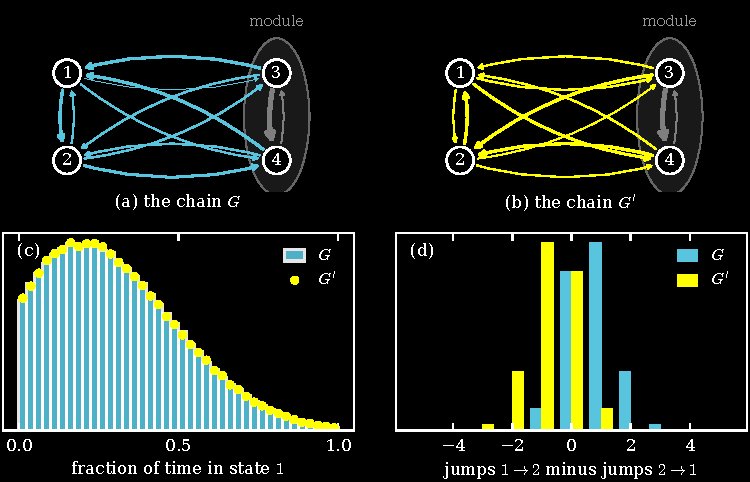
\includegraphics[width=\textwidth]{fig_twins}
\caption{The two chains of Example~\ref{ex:four}. (a), (b) The rates, with
thicker arrows for larger rates. The gray arrows inside the module are the
same in both chains, and every other rate differs. (c) The fraction of time in
state $1$ up to time $t=4$, from $4\cdot10^5$ simulated paths of each chain.
The two histograms agree, as they must. (d) The number of jumps from $1$ to
$2$ minus the number from $2$ to $1$ on the same paths. This sees the order of
the visits, and it tells the chains apart at once.}
\label{fig:twins}
\end{figure}

When both parts apply, and neither the inside chain nor the lumped chain is
reversible, we get four chains with the same counts, namely $G$, the chain with
only the outside reversed, the chain with only the inside reversed, and the
chain with both reversed (checked on six states with a stationary start, where
the last one is $\hat G$).

\section{What is lost}

Now let $G=TQ$, with $\mu$ known and positive and every $Q_{ij}>0$. We compare
the Fisher information about $Q$ in the full path on $[0,1]$, written
$I_{\mathrm{path}}$, with the information in $L(1)$, written $I_L$. Here
$c_{ij}=\mu_iQ_{ij}+\mu_jQ_{ji}$ and $q_i=\sum_jQ_{ij}$ are functions of $Q$, and
for three states we put
\[
\tau_{ijk}=\sum_{(x,y,z)}\mu_xQ_{xy}Q_{yz}
=\sum_{y}\frac{c_{xy}c_{yz}+J_{xy}J_{yz}}{2\mu_y},
\]
where the first sum is over the six orders of $\{i,j,k\}$ and in the second $x$
and $z$ are the two states other than $y$.

\begin{theorem}[rare switches]\label{thm:info}
As $T\to0$,
\[
I_{\mathrm{path}}=T\operatorname{diag}\Bigl(\frac{\mu_i}{Q_{ij}}\Bigr)+O(T^2),
\qquad
I_L=T\sum_{i<j}\frac{\nabla c_{ij}\nabla c_{ij}^{\top}}{c_{ij}}+O(T^2).
\]
So the efficiencies (the eigenvalues of $I_{\mathrm{path}}^{-1}I_L$) split in
half, with $\binom d2$ of them tending to $1$ and $\binom d2$ tending to $0$. The
counts are first-order efficient for every two-way flow $c_{ij}$ and carry no
first-order information about any net flow. For a direction $v$ with
$v\cdot\nabla c_{ij}=0$ for all pairs,
\begin{equation}\label{eq:second}
v^{\top}I_Lv=T^2\Bigl[\sum_i\mu_i(v\cdot\nabla q_i)^2
+\sum_{i<j<k}\frac{(v\cdot\nabla\tau_{ijk})^2}{2\tau_{ijk}}\Bigr]+O(T^3).
\end{equation}
\end{theorem}
\begin{proof}
The score of the path for $Q_{ij}$ is $s_{ij}=N_{ij}/Q_{ij}-TL_i$, where $N_{ij}$
counts the jumps from $i$ to $j$, and $I_L=\E[\bar s\bar s^{\top}]$ with
$\bar s=\E[s\mid L]$. Since $\E N_{ij}=T\mu_iQ_{ij}+O(T^2)$, the first claim
follows. For the second we sort by the face of the simplex that holds $L$. The
chance of three or more jumps is $O(T^3)$, and so is the second moment of the
score on that event.

\emph{A vertex.} $L=e_i$ means no jump, so $\bar s=-T\nabla q_i$ there, with
probability $\mu_i+O(T)$. This contributes $T^2\mu_i\nabla q_i\nabla q_i^{\top}$.

\emph{An edge.} Given $L$ on the edge of $i$ and $j$, up to a relative error
$O(T)$ that is uniform along the edge, the path made one jump, from $i$ to $j$
with probability $f_{ij}/c_{ij}$ and from $j$ to $i$ otherwise. So
$\bar s_{ij}=\mu_i/c_{ij}+O(T)$ and $\bar s_{ji}=\mu_j/c_{ij}+O(T)$, that is,
$\bar s=\nabla c_{ij}/c_{ij}+O(T)$. The edge has probability $Tc_{ij}+O(T^2)$.
This contributes $T\nabla c_{ij}\nabla c_{ij}^{\top}/c_{ij}+O(T^2)$, and
$O(T^3)$ in a direction $v$ with $v\cdot\nabla c_{ij}=0$.

\emph{A triangle.} Given $L$ in the open face of $i$, $j$ and $k$, up to a
uniform relative error $O(T)$ the path made two jumps in one of six orders. Each
order fits every point of the face, and the order $(x,y,z)$ has probability
$\mu_xQ_{xy}Q_{yz}/\tau_{ijk}$. Since $\tau_{ijk}$ is linear in each rate,
$\bar s=\nabla\tau_{ijk}/\tau_{ijk}+O(T)$. The face has probability
$T^2\tau_{ijk}/2+O(T^3)$, because the two jump times fill half of the unit
square. This contributes the last term of~\eqref{eq:second}.

For the efficiencies, in the coordinates $f_{ij}$ the matrix
$I_{\mathrm{path}}^{-1}I_L$ tends to a block for each pair, equal to
$\operatorname{diag}(f_{ij},f_{ji})$ times the all-ones matrix over $c_{ij}$,
with eigenvalues $1$ and $0$.
\end{proof}

When switches are rare, a typical path that tells us anything has one jump. The
counts then say which two states and when, but not which way. This is why they
keep the two-way flows and lose the net flows. The net flows come back at the
next order from two places in~\eqref{eq:second}, the paths that never move (their
number gives the exit rates) and the paths that visit three states.

\begin{theorem}[stationary start]\label{thm:singular}
Let the start be the stationary law, and use the coordinates $(\pi,c,J)$ for
$Q$, where $J$ obeys Kirchhoff's law at every state. Then the law of $L(t)$ is
an even function of $J$. So at every reversible chain, and for every $t$, the
information matrix of $L(t)$ vanishes on the $J$ directions, a space of dimension
$\binom{d-1}2$.
\end{theorem}
\begin{proof}
Reversal sends $(\pi,c,J)$ to $(\pi,c,-J)$ and keeps the law
(Proposition~\ref{prop:reversal}). The derivative of an even function vanishes
at $0$, so the score in every $J$ direction is zero at $J=0$. The $J$ directions
are the cycle space of the complete graph, of dimension
$\binom d2-(d-1)$.
\end{proof}

\begin{remark}
Near a reversible chain the law depends on $J$ through quadratic terms such as
the one in $\tau_{ijk}$. So from $n$ copies of the counts one should expect to
learn $J^2$ at the usual rate, hence $|J|$ only at rate $n^{-1/4}$ near $J=0$,
and never its sign. We have not proved this. (Rates of this kind are known for
models whose information matrix loses rank by one~\cite{rcbr2000}, which is
the case of three states. There the model is assumed identifiable, and ours is
not, because of the sign.) For three states and $T=2$ the smallest
eigenvalue of the information matrix is $0.94\,j^2$, $0.96\,j^2$ at $j=0.04$,
$0.02$, where $j$ is the flow around the triangle.
\end{remark}

The crossings of Paper~C sit at the other end, where $T$ is of order $\log N$
and so is large. There the counts keep the stationary law and, as far as we can
see, nothing else. The first half of this is a theorem. Let $\pi$ be the
stationary law of $Q$, let $Z=(\one\pi^{\top}-Q)^{-1}-\one\pi^{\top}$, and let
$\Gamma=\operatorname{diag}(\pi)Z+Z^{\top}\operatorname{diag}(\pi)$, the
asymptotic covariance of the occupation times (so $\operatorname{Cov}L(1)
=\Gamma/T+O(T^{-2})$ for the generator $TQ$).

\begin{theorem}[long horizons]\label{thm:long}
Let $Q$ be irreducible with every $Q_{ij}>0$, let the start be any fixed law or
the stationary law, and let $D=\operatorname{diag}(\pi_i/Q_{ij})$. Write $\pi'$
for the matrix of the derivatives $\partial\pi_k/\partial Q_{ij}$.
\begin{enumerate}[(a),itemsep=1pt]
\item $\pi'D^{-1}\pi'^{\top}=\Gamma$. In words, the Cram\'er--Rao bound of the
 full path for $\pi$ is the variance of the occupation fractions.
\item As $T\to\infty$, $I_{\mathrm{path}}=TD+O(1)$ and
 $I_L\succeq T\,\pi'^{\top}\Gamma^{+}\pi'-O(1)$, where $\Gamma^{+}$ is the
 inverse of $\Gamma$ on the vectors with sum zero. So $d-1$ of the efficiencies
 tend to $1$.
\end{enumerate}
\end{theorem}
\begin{proof}
(a) We compute both sides as quadratic forms in a vector $\eta$ and find the
same sum over pairs. We use the three facts $Z\one=0$, $\pi^{\top}Z=0$ and
$-QZ=I-\one\pi^{\top}$, which follow from
$(\one\pi^{\top}-Q)(Z+\one\pi^{\top})=I$. Differentiating $\pi^{\top}Q=0$ gives
$d\pi^{\top}Q=-\pi^{\top}dQ$. Multiply by $Z$ on the right and use
$d\pi^{\top}\one=0$. This gives $d\pi^{\top}=\pi^{\top}(dQ)Z$. Raising $Q_{ij}$ (and lowering $Q_{ii}$)
gives $\partial\pi/\partial Q_{ij}=\pi_i(Z_{j\cdot}-Z_{i\cdot})$. So for a
vector $\eta$ and $u=Z\eta$, the entry of $\pi'^{\top}\eta$ at $(i,j)$ is
$\pi_i(u_j-u_i)$, and
\[
 \eta^{\top}\pi'D^{-1}\pi'^{\top}\eta=\sum_{i\ne j}\frac{Q_{ij}}{\pi_i}\,
 \pi_i^2(u_j-u_i)^2=\sum_{i\ne j}\pi_iQ_{ij}(u_j-u_i)^2 .
\]
On the other side $\eta^{\top}\Gamma\eta=2\sum_i\pi_i\eta_iu_i$. Here
$-Qu=\eta-(\pi\cdot\eta)\one$ and $\pi\cdot u=0$, so
$\eta^{\top}\Gamma\eta=-2\sum_i\pi_iu_i(Qu)_i$. Now expand the squares in the
display. The terms with $u_i^2$ and with $u_j^2$ each give $\sum_i\pi_iq_iu_i^2$
(the second by $\pi^{\top}Q=0$), and the cross terms give
$-2\sum_i\pi_iu_i\bigl((Qu)_i+q_iu_i\bigr)$. The sum is the same number.

We note for part (b) that $\Gamma$ is positive definite on the vectors with sum
zero. Indeed the display vanishes only if $u$ is constant. Then $u=0$ because
$\pi\cdot u=0$, and so $\eta=(\pi\cdot\eta)\one$.

(b) The first claim is as in Theorem~\ref{thm:info}. The path information is
diagonal with entries $T\,\E L_i(1)/Q_{ij}$, and $\E L_i(1)=\pi_i+O(1/T)$. (A
stationary start adds the information in the first state, which is $O(1)$.)

For the second claim we bound $I_L$ from below by what the mean of $L$ alone
tells us. Let $m$ and $V$ be the mean and the covariance of $L=L(1)$ under the
generator $TQ$, and let $s$ be the score of $L$. Differentiating $\E L=m$ gives
$\E[(L-m)s^{\top}]=m'$. So the covariance matrix of the pair $(L,s)$ has the
blocks $V$, $m'$ and $I_L$, and it is positive semidefinite. Its Schur
complement gives $I_L\succeq m'^{\top}V^{+}m'$, where $V^{+}$ is the
pseudoinverse of $V$. (The coordinates of $L$ sum to $1$, so $V\one=0$ and
$V^{+}$ lives on the vectors with sum zero.) Now $e^{tQ}-\one\pi^{\top}$ decays
exponentially, locally uniformly in $Q$ and together with its derivatives in
$Q$. So
\[
m=\pi+O(1/T),\qquad m'=\pi'+O(1/T),\qquad V=\Gamma/T+O(T^{-2}).
\]
Since $\Gamma$ is invertible on the vectors with sum zero, so is $V$ for large
$T$, with $V^{+}=T\,\Gamma^{+}+O(1)$. This gives the bound.

Finally we count the efficiencies that tend to $1$. The nonzero eigenvalues of
$D^{-1}\pi'^{\top}\Gamma^{+}\pi'$ are those of
$\Gamma^{+}\pi'D^{-1}\pi'^{\top}$, which is $\Gamma^{+}\Gamma$ by (a). So they
are $1$ with multiplicity $d-1$. The eigenvalues of $I_{\mathrm{path}}^{-1}I_L$
can only go up when $I_L$ does, so by the two estimates of (b) the largest
$d-1$ of them are at least $1-O(1/T)$. Every efficiency is at most $1$, because
$L$ is a function of the path.
\end{proof}

So over a long horizon the counts estimate the stationary law as well as the
full path does. That the occupation fractions are an efficient estimate of
$\pi$ is classical (see~\cite{albert1962} for the path likelihood
and~\cite{gw1994} for efficiency). Part (a) is the identity behind it. The
other $(d-1)^2$ efficiencies appear to decay like $1/T$ (Table~\ref{tab:eff}),
but we have not proved that they tend to $0$.

\begin{figure}[t]
\centering
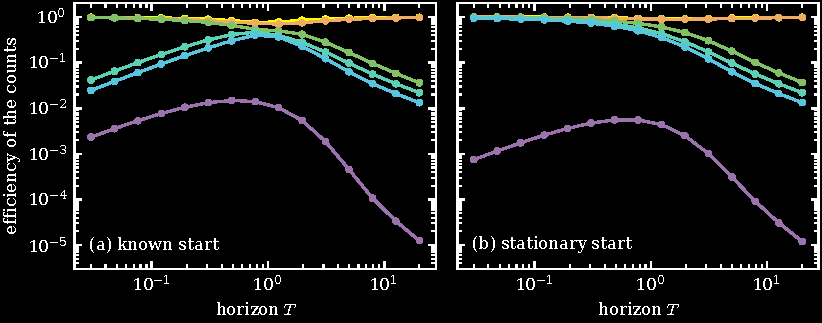
\includegraphics[width=\textwidth]{fig_information}
\caption{The six efficiencies of the counts against the horizon $T$, for the
chain of Table~\ref{tab:eff}. For few switches they split as in
Theorem~\ref{thm:info}. Three are lost with a known start, and only the flow
around the triangle with a stationary start. For many switches two tend to $1$
(Theorem~\ref{thm:long}) and the others fall off like $1/T$.}
\label{fig:information}
\end{figure}

\begin{table}[ht]\centering\small
\begin{tabular}{rll}
\toprule
$T$ & known start & stationary start\\
\midrule
$0.05$ & $0.98,\ 0.97,\ 0.95,\ 0.07,\ 0.04,\ 0.004$ & $1.00,\ 1.00,\ 0.98,\ 0.95,\ 0.92,\ 0.001$\\
$1$ & $0.75,\ 0.72,\ 0.50,\ 0.43,\ 0.42,\ 0.012$ & $0.92,\ 0.90,\ 0.67,\ 0.50,\ 0.42,\ 0.005$\\
$20$ & $0.99,\ 0.97,\ 0.04,\ 0.02,\ 0.01,\ 10^{-5}$ & $0.99,\ 0.98,\ 0.04,\ 0.02,\ 0.01,\ 10^{-5}$\\
\bottomrule
\end{tabular}
\caption{The six efficiencies of the counts for one chain on three states
(exact, from the $N$-step chain with $N$ at least $240$). For small $T$ three
are lost with a known start, as in Theorem~\ref{thm:info}, and only the flow
around the triangle with a stationary start. For large $T$ only two survive
(the stationary law, Theorem~\ref{thm:long}). This last regime is the one of
Paper~C's crossings, where $T$ is of order $\log N$.}
\label{tab:eff}
\end{table}

\section{Checks and open questions}

Each statement above was checked numerically in the scripts next to this note.
\begin{itemize}[itemsep=1pt]
\item \texttt{check\_identifiability.py}. Reversal agrees to $10^{-15}$ for
 $d=3,4,5$. The map from $G$ to the law has full rank at random points for
 $d=2,3,4$ with a known start, a stationary start and a start at one state. At
 reversible chains with a stationary start the rank drops by exactly
 $\binom{d-1}2$ for $d=3,4,5$. Block reversal at a cut state works when the
 return rates are equal and fails (by $2\cdot10^{-3}$) when they are not.
\item \texttt{check\_lumping\_decoder.py}. Example~\ref{ex:four}. The recipe of
 the remark after Corollary~\ref{cor:generic} returns one generator for a random
 start and two for a stationary start, for $d=3,4,5$. For the $N$-step chain on
 three states the map from $P$ to the law of $K_N$ has full rank once $N\ge3$.
\item \texttt{check\_information.py}. The two leading terms of
 Theorem~\ref{thm:info} (the first to within $0.017$ at $T=0.025$, the second
 within $3\%$ at $T=0.02$ and still converging), Theorem~\ref{thm:singular} and
 Table~\ref{tab:eff}.
\item \texttt{check\_entropy.py}. Theorem~\ref{thm:entropy}. The entropy
 production is recovered from the function $r$ alone, to four digits, for
 $d=3,4,5$ and both kinds of start. Chains with the same counts have the same
 $\sigma$, and the triangle affinities are recovered from the principal minors
 of orders up to three.
\item \texttt{check\_rigidity.py}. Part (b) of Theorem~\ref{thm:lumping} and
 Example~\ref{ex:inside} (the laws agree to $10^{-15}$ for $d=4,5,7$). In each
 tie both sets of minors of Proposition~\ref{prop:minors} agree. For a random
 chain with a start that is not stationary, the reversal has the same minors of
 $G$ but not of $G-\one\mu^{\top}$, and the laws differ.
\end{itemize}

What we do not know.
\begin{enumerate}[1.,itemsep=1pt]
\item Is every tie built from the two reversals of Theorem~\ref{thm:lumping}?
 For a chain with no cut the answer is in Theorem~\ref{thm:rigid}, up to
 deciding~\eqref{eq:startend}. For a chain with a cut, the results
 of~\cite{cggr2025} list every $G'$ with the same principal minors as $G$, so
 what is left is to find which of them also pass the test with
 $G-\one\mu^{\top}$. For four states with every rate positive, one step across
 one cut is enough to reach every such $G'$~\cite[Lemma~3.1]{cggr2025}.
\item When does~\eqref{eq:startend} hold? A stationary start and
 Example~\ref{ex:inside} are the cases we know.
\item Does Theorem~\ref{thm:horizon} have a form for the $N$-step chain? The
 proof uses that exponentials of algebraic functions do not cancel, and powers
 of algebraic functions can.
\item The large $T$ row of Table~\ref{tab:eff}. By Theorem~\ref{thm:long},
 $d-1$ efficiencies tend to $1$. We expect the rest to decay like $1/T$.
\item A start at one state. The rank check says almost every chain is
 recovered, and the pair formulas change because some $\mu_i$ vanish.
 (Proposition~\ref{prop:minors} and Theorem~\ref{thm:rigid} do not need
 $\mu_i>0$.)
\end{enumerate}

\paragraph{What is in the literature.} A search (not a full review) found the
following. The algebra of Section~\ref{sec:rigid} and of the polynomial $\chi_0$ in Section~\ref{sec:lumping}
is the theory of matrices with equal principal
minors~\cite{hl1984,loewy1986,alahmadieh2026,cggr2025}. We did not find
Theorem~\ref{thm:horizon}, the role of the start law (the unordered pairs of
flows in Theorem~\ref{thm:pairs}, the second matrix in
Proposition~\ref{prop:minors}, condition~\eqref{eq:startend}, and
Theorem~\ref{thm:lumping} as a statement about the law of $L(t)$), or
Theorems~\ref{thm:entropy}, \ref{thm:info} and~\ref{thm:singular}. Work on aggregate data from
Markov chains and on the embedding problem observes something else, namely how
many of a population sit in each state at given times. Work on aggregated
Markov processes (see~\cite{fr1986}) observes a lumped path over time, with
its order, and not the total times. We have not read
\cite{hl1984} and~\cite{loewy1986} themselves. Their statements are taken from
\cite{alahmadieh2026} and~\cite{cggr2025}, which agree.

\begin{thebibliography}{99}\small
\bibitem{albert1962} A.~Albert, Estimating the infinitesimal generator of a
 continuous time, finite state Markov process, \emph{Ann. Math. Statist.}
 \textbf{33} (1962), 727--753.
\bibitem{alahmadieh2026} A.~Al~Ahmadieh, On the fibers of the principal minor
 map and an application to stable polynomials, \emph{J. Algebra} \textbf{685}
 (2026), 46--61. arXiv:2309.00806.
\bibitem{ax1971} J.~Ax, On Schanuel's conjectures, \emph{Ann. of Math.}
 \textbf{93} (1971), 252--268.
\bibitem{cggr2025} A.~Chatterjee, S.~Ghosh, R.~Gurjar and R.~Raj,
 Characterizing and testing principal minor equivalence of matrices,
 \emph{Proc. 57th ACM Symposium on Theory of Computing} (2025), 1067--1078.
 arXiv:2410.01961.
\bibitem{dlp2016} A.~B.~Duncan, T.~Leli\`evre and G.~A.~Pavliotis, Variance
 reduction using nonreversible Langevin samplers, \emph{J. Stat. Phys.}
 \textbf{163} (2016), 457--491.
\bibitem{fr1986} D.~R.~Fredkin and J.~A.~Rice, On aggregated Markov processes,
 \emph{J. Appl. Probab.} \textbf{23} (1986), 208--214.
\bibitem{gw1994} P.~E.~Greenwood and W.~Wefelmeyer, Nonparametric estimators
 for Markov step processes, \emph{Stochastic Process. Appl.} \textbf{52}
 (1994), 1--16.
\bibitem{hl1984} D.~J.~Hartfiel and R.~Loewy, On matrices having equal
 corresponding principal minors, \emph{Linear Algebra Appl.} \textbf{58}
 (1984), 147--167.
\bibitem{kjz2017} M.~Kaiser, R.~L.~Jack and J.~Zimmer, Acceleration of
 convergence to equilibrium in Markov chains by breaking detailed balance,
 \emph{J. Stat. Phys.} \textbf{168} (2017), 259--287.
\bibitem{kelly1979} F.~P.~Kelly, \emph{Reversibility and Stochastic Networks},
 Wiley, Chichester, 1979.
\bibitem{loewy1986} R.~Loewy, Principal minors and diagonal similarity of
 matrices, \emph{Linear Algebra Appl.} \textbf{78} (1986), 23--64.
\bibitem{mnw2008} C.~Maes, K.~Neto\v{c}n\'y and B.~Wynants, On and beyond
 entropy production: the case of Markov jump processes, arXiv:0709.4327.
\bibitem{mr2013} M.~B.~Marcus and J.~Rosen, A sufficient condition for the
 continuity of permanental processes with applications to local times of Markov
 processes, \emph{Ann. Probab.} \textbf{41} (2013), 671--698.
\bibitem{rcbr2000} A.~Rotnitzky, D.~R.~Cox, M.~Bottai and J.~Robins,
 Likelihood-based inference with singular information matrix, \emph{Bernoulli}
 \textbf{6} (2000), 243--284.
\bibitem{schnakenberg1976} J.~Schnakenberg, Network theory of microscopic and
 macroscopic behavior of master equation systems, \emph{Rev. Modern Phys.}
 \textbf{48} (1976), 571--585.
\end{thebibliography}

\end{document}
